\documentclass{article}
\usepackage{listings}
\usepackage{graphicx}
\usepackage{float}

\DeclareGraphicsExtensions{.jpeg,.png}
\graphicspath{ {/Users/llaryssa/Documents/Stevens/CS532-3DCV/CS532-assignments/assignment5/imgs/} }


\begin{document}

\centerline{\sc \large CS 532: Homework Assignment 5}
\vspace{.3pc}
\centerline{Alana Laryssa Seabra A Santos}
\centerline{\it 11/18/2015}
\vspace{.6pc}

\section{Voxel-based reconstruction from silhouettes}

The 3D model below was reconstructed using a initial voxel grid with $x$ range equals to -2.5m to 2.5m, $y$ from -3m to 3m and $z$ from 0 to 2.5m. With resolution 0.01, this gives a number of 75576351 initial voxels. In the end, there were 98584 voxels left to represent the dancer.

\begin{figure}[H]
  \caption{dancer0.ply}
  \centering
    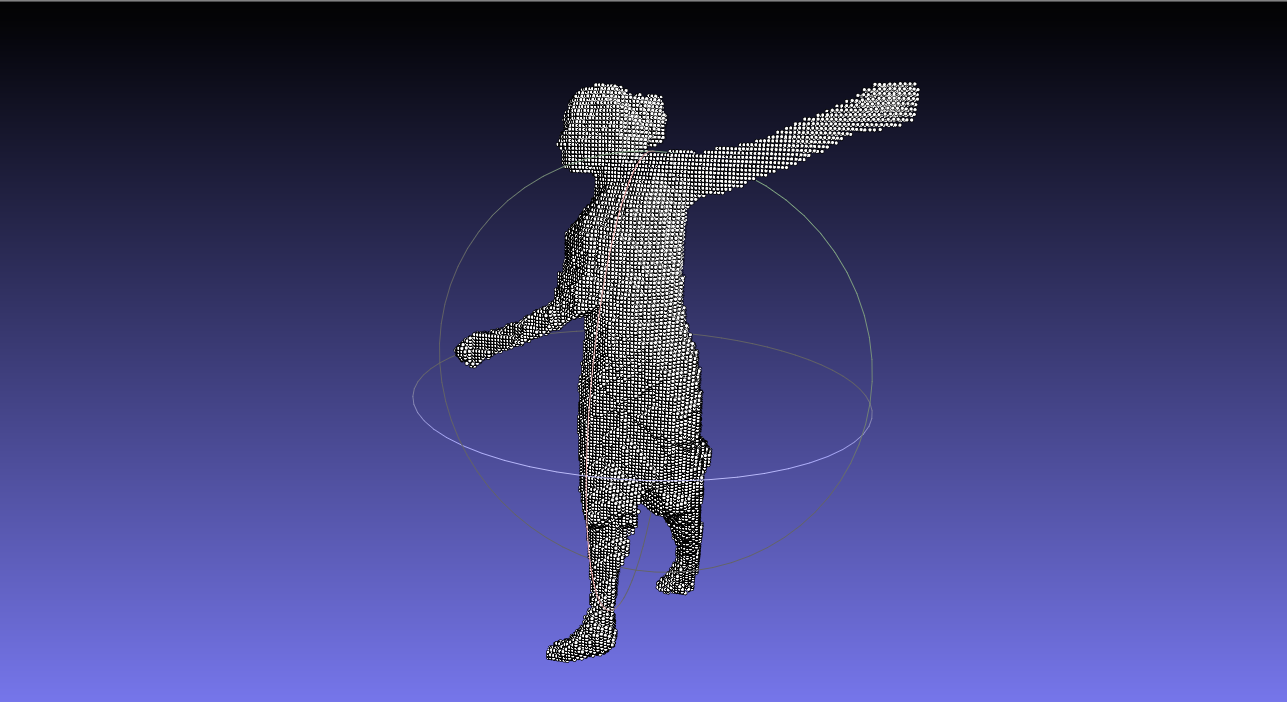
\includegraphics[scale=0.14]{voxel1}
\end{figure}

\begin{figure}[H]
  \caption{dancer0.ply}
  \centering
    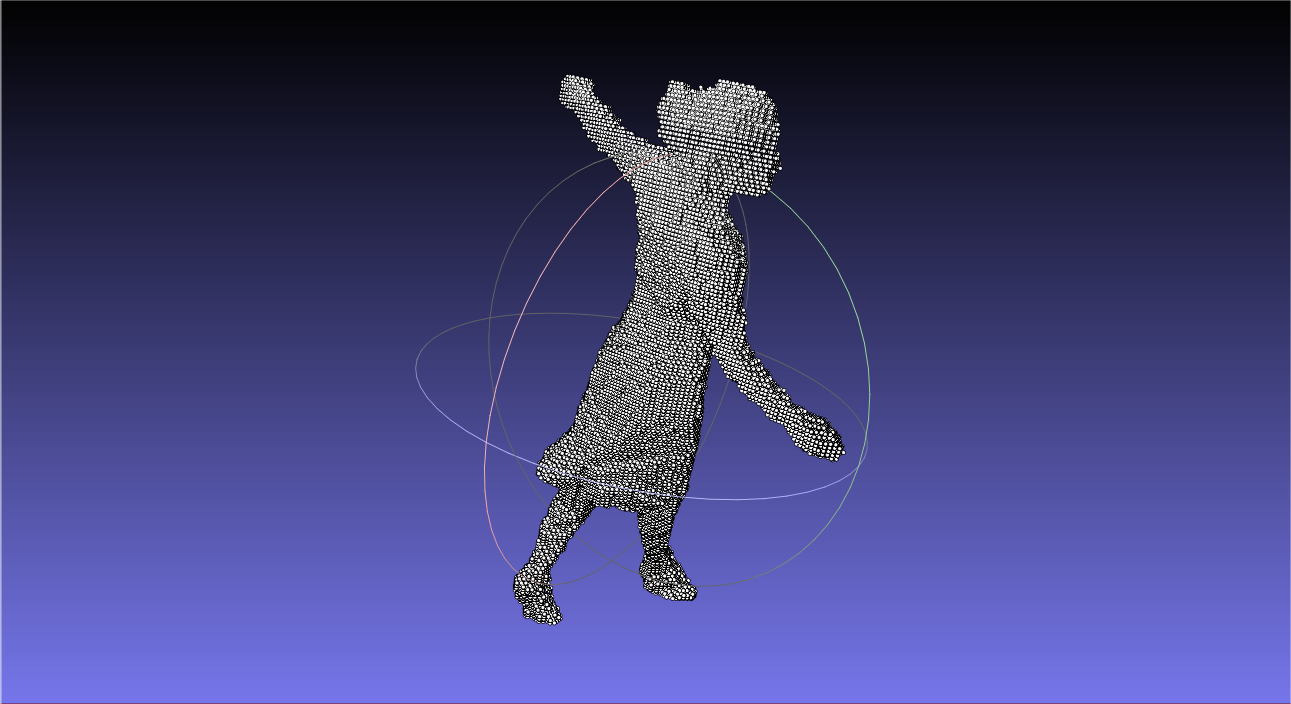
\includegraphics[scale=0.14]{voxel2}
\end{figure}

\begin{figure}[H]
  \caption{dancer0.ply}
  \centering
    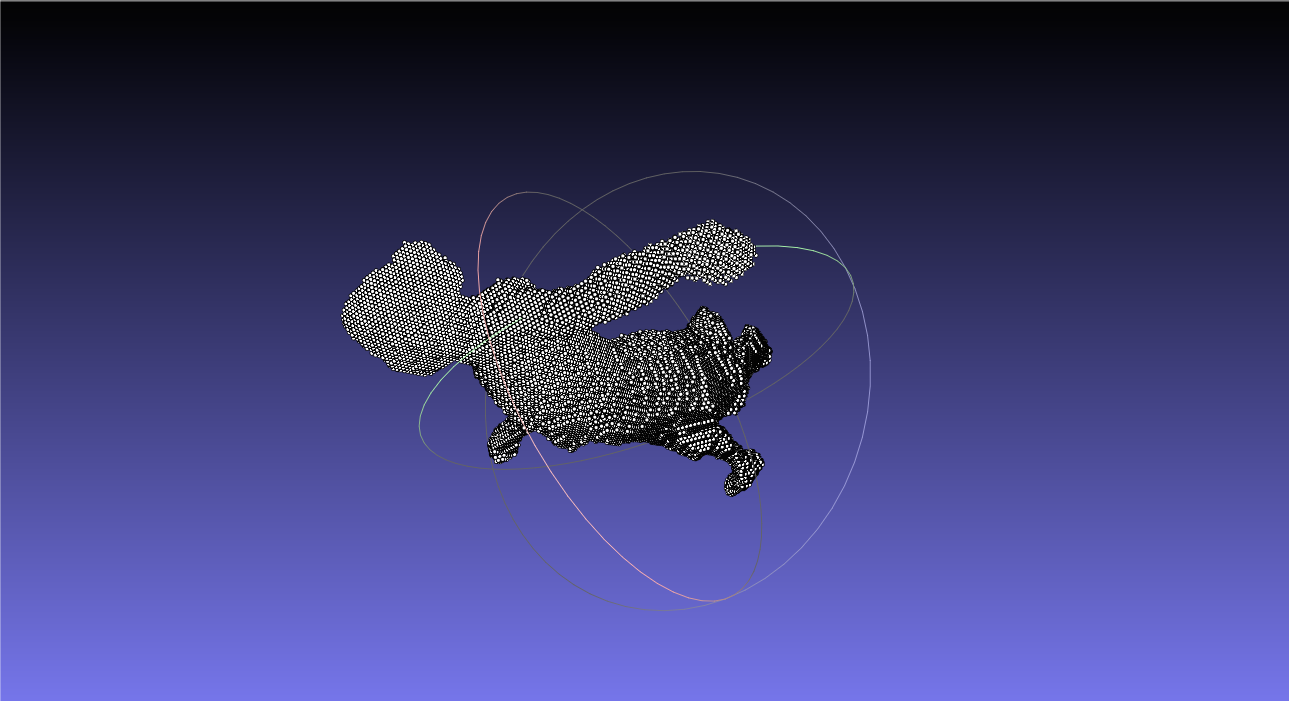
\includegraphics[scale=0.14]{voxel3}
\end{figure}

\section{Coloring}

First, I tried to color all the points with color information from the first image. As expected, the up-front part of the model was perfect, but rest was bad. Then I tried to color with a blend of all the cameras, just getting the mean off all colors. The results are below:

\begin{figure}[H]
  \caption{dancer1.ply}
  \centering
    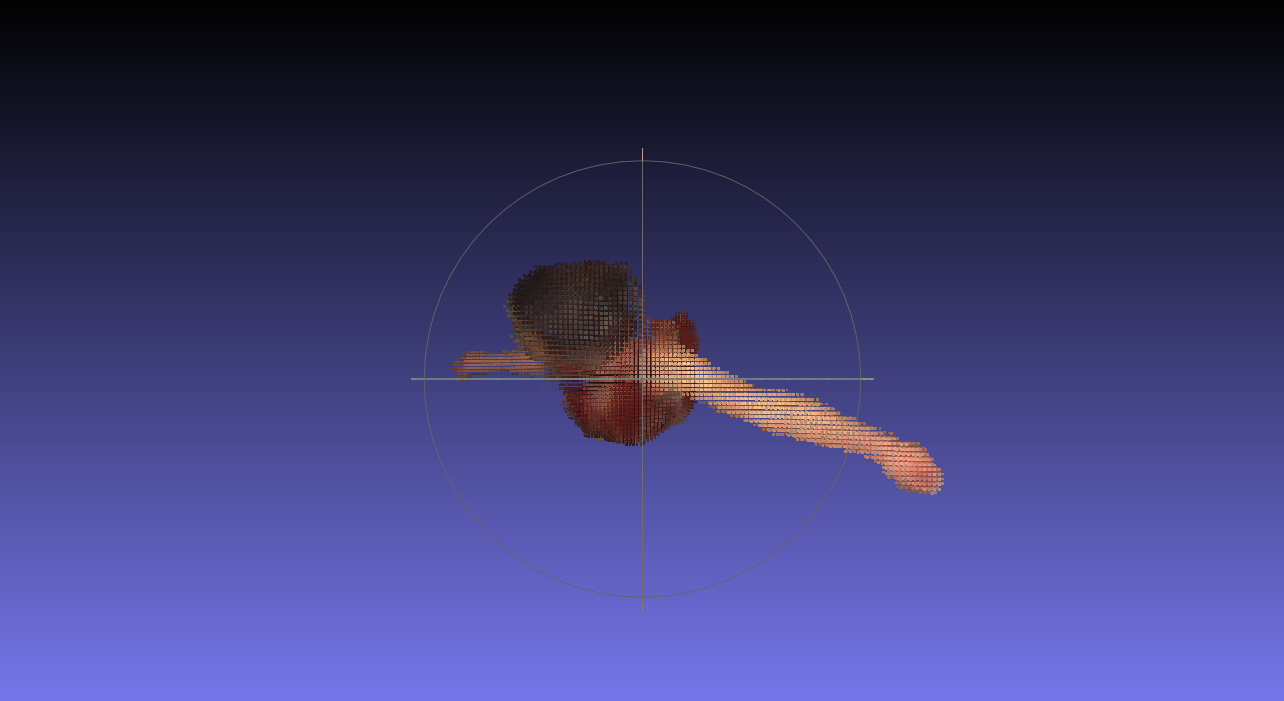
\includegraphics[scale=0.15]{mean1}
\end{figure}

\begin{figure}[H]
  \caption{dancer1.ply}
  \centering
    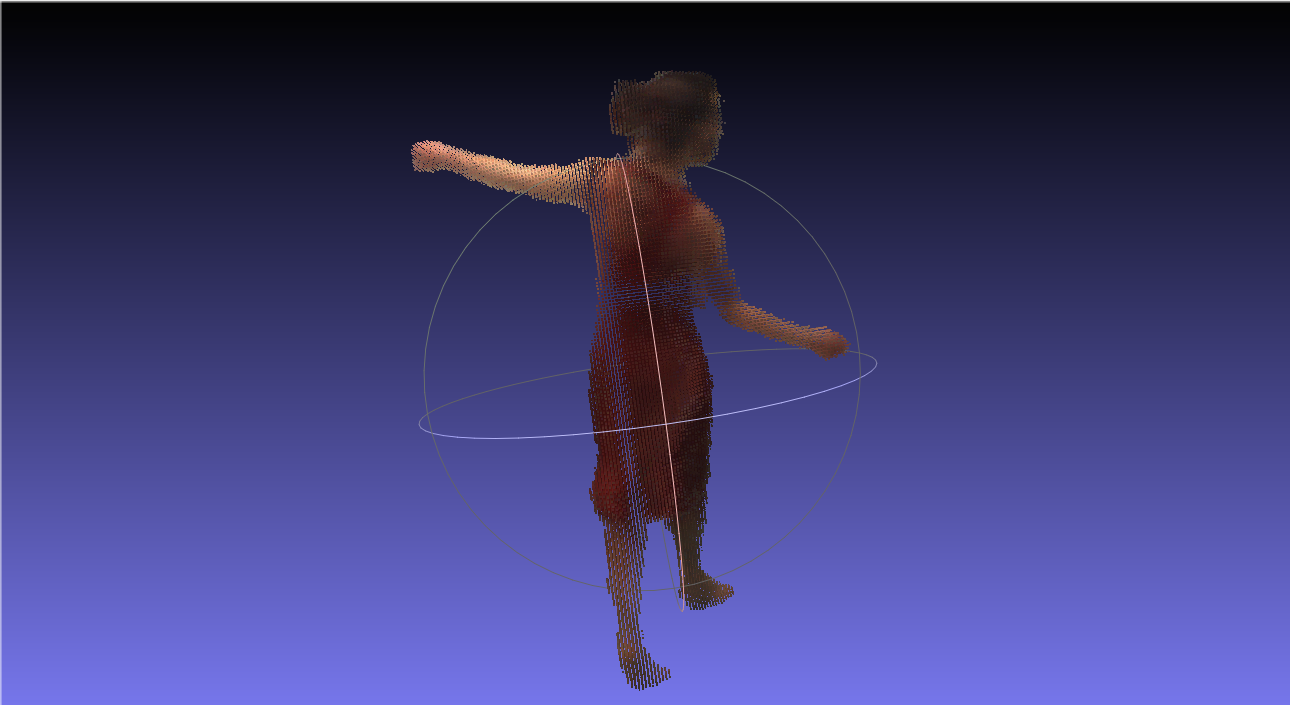
\includegraphics[scale=0.15]{mean2}
\end{figure}

\begin{figure}[H]
  \caption{dancer1.ply}
  \centering
    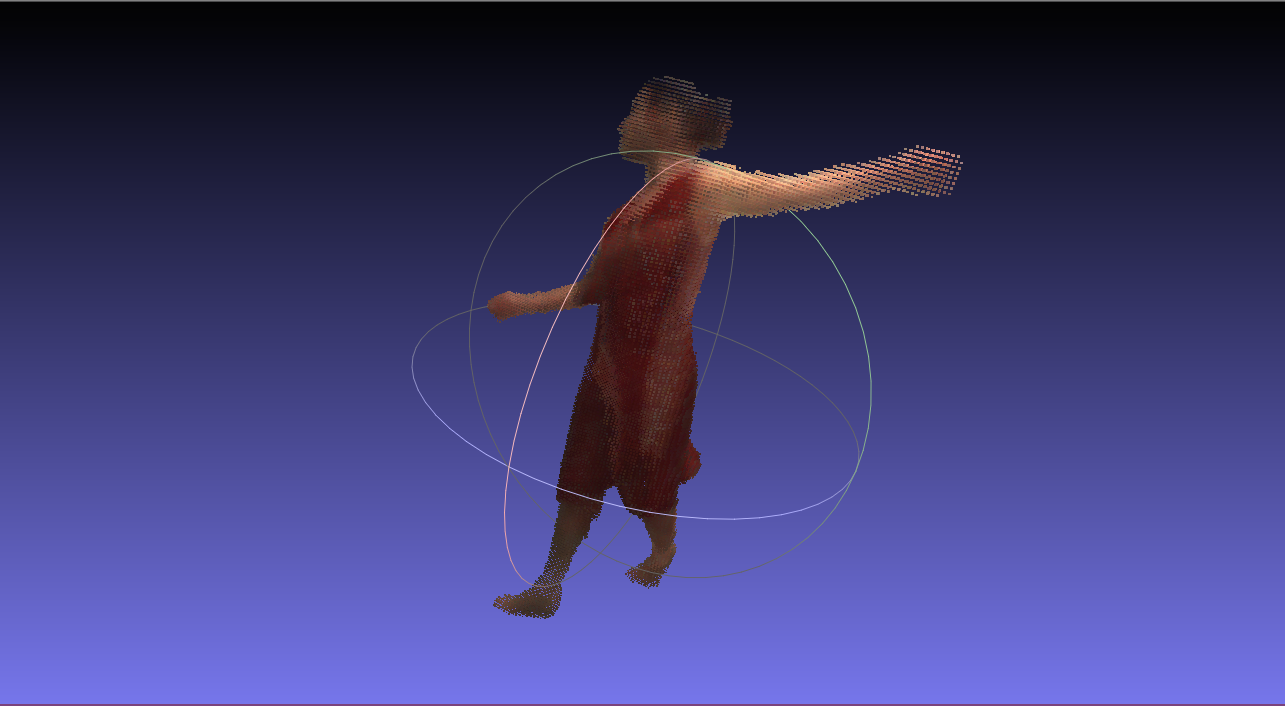
\includegraphics[scale=0.15]{mean3}
\end{figure}

The results are not too bad, but also aren't good. Then I tried to find the best camera view for each point, and I saw somewhere online that I could do that by comparing the normal vector of the point with the camera view vector. So, I used a Matlab code by Zachary Taylor to find the normals of the points. Then, I compared them with the cameras $z-axis$ and kept the index of the camera that provided minimum angle between these vectors. The result didn't came out as good as I expected. But I imagine that if I could estimate the normals only at the surface points, I would get better results.

\begin{figure}[H]
  \caption{dancer3.ply}
  \centering
    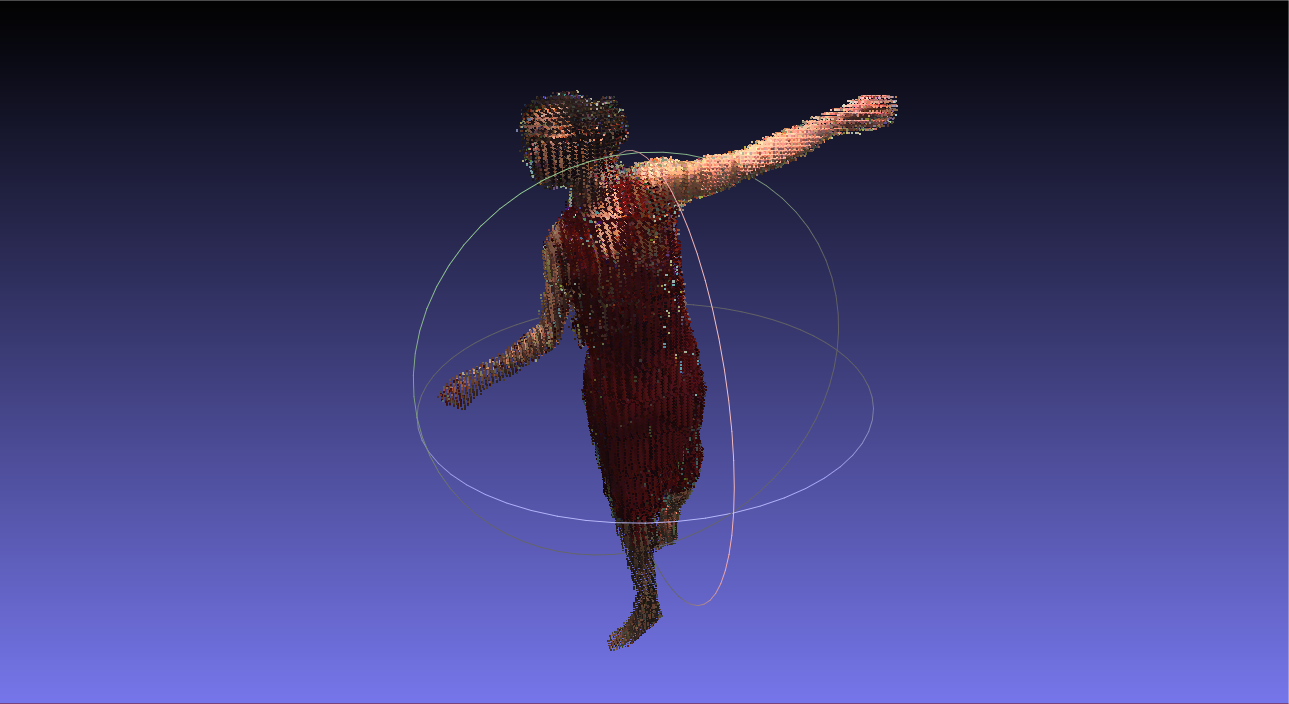
\includegraphics[scale=0.16]{try1}
\end{figure}

\begin{figure}[H]
  \caption{dancer3.ply}
  \centering
    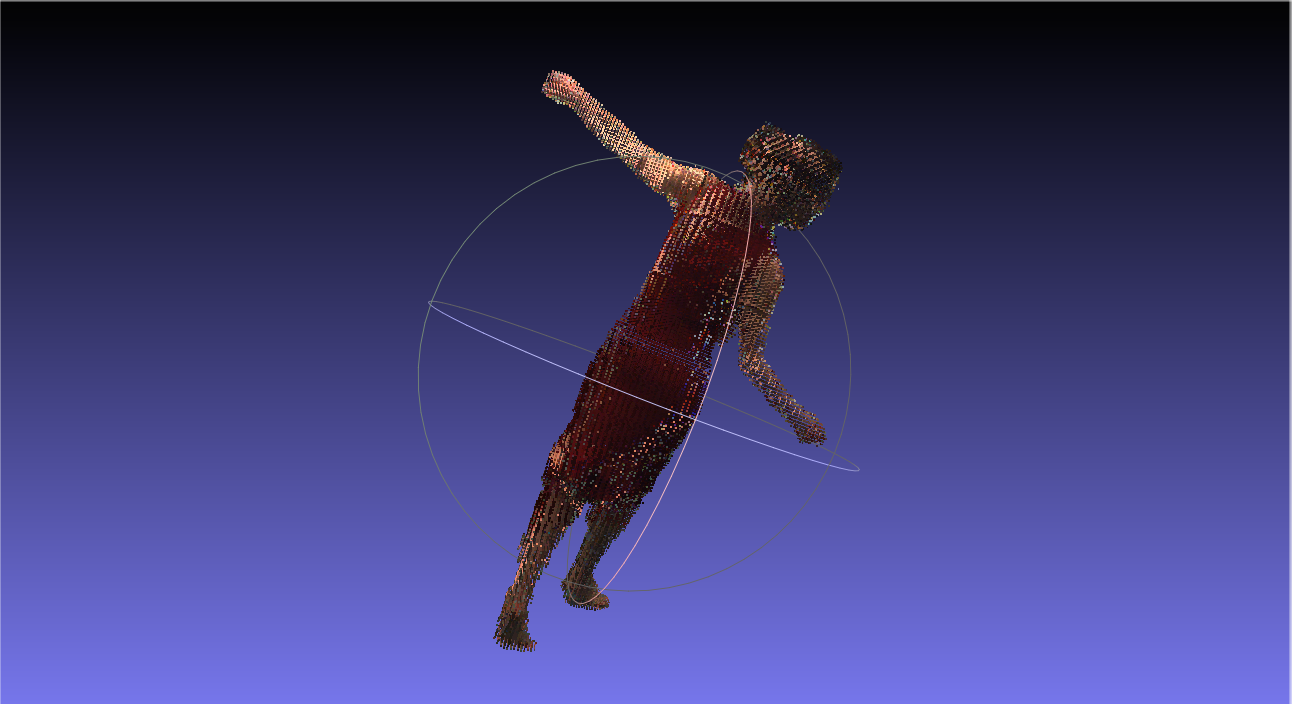
\includegraphics[scale=0.16]{try2}
\end{figure}

\begin{figure}[H]
  \caption{dancer3.ply}
  \centering
    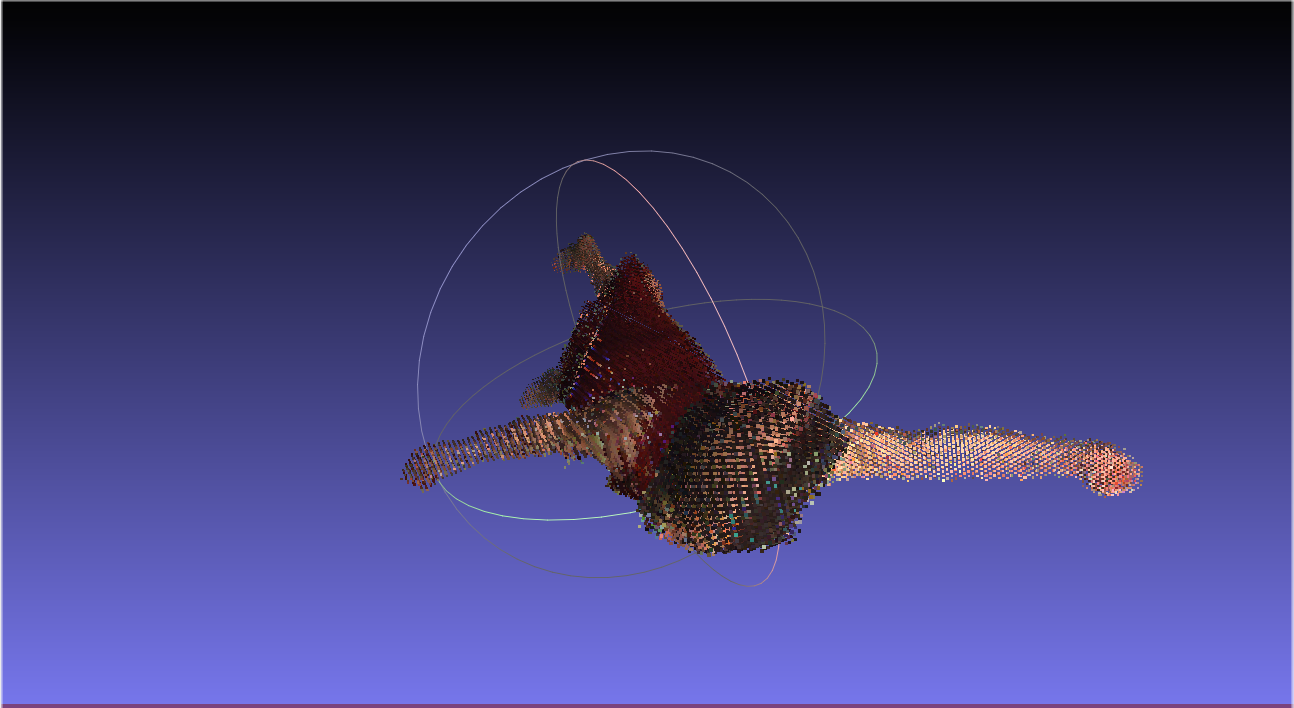
\includegraphics[scale=0.15]{try3}
\end{figure}


\end{document}


